%%%%%%%% ICML 2025 EXAMPLE LATEX SUBMISSION FILE %%%%%%%%%%%%%%%%%

\documentclass{article}

% Recommended, but optional, packages for figures and better typesetting:
\usepackage{microtype}
\usepackage{graphicx}
\usepackage{subfigure}
\usepackage{booktabs} % for professional tables
\usepackage{wrapfig}    % wrap figures

% Code listings
\usepackage{listings}
\usepackage{xcolor}

\lstdefinestyle{pyicml}{
  language=Python,
  basicstyle=\ttfamily\footnotesize,
  numbers=left,
  numberstyle=\tiny,
  stepnumber=1,
  numbersep=6pt,
  showstringspaces=false,
  columns=fullflexible,      % better line breaks in two-column
  keepspaces=true,
  breaklines=true,
  breakatwhitespace=true,
  tabsize=2,
  frame=single,
  framerule=0.2pt,
  rulecolor=\color{black!20},
  keywordstyle=\bfseries,
  commentstyle=\itshape\color{black!55},
  stringstyle=\color{black},
}


% hyperref makes hyperlinks in the resulting PDF.
% If your build breaks (sometimes temporarily if a hyperlink spans a page)
% please comment out the following usepackage line and replace
% \usepackage{icml2025} with \usepackage[nohyperref]{icml2025} above.
\usepackage{hyperref}
% algorithm/algpseudocode already loaded by icml2025.sty


% Attempt to make hyperref and algorithmic work together better:
% Use the following line for the initial blind version submitted for review:
% \usepackage{icml2025}

% If accepted, instead use the following line for the camera-ready submission:
\usepackage[accepted]{icml2025}

% For theorems and such
\usepackage{amsmath}
\usepackage{amssymb}
\usepackage{mathtools}
\usepackage{amsthm}

% if you use cleveref..
\usepackage[capitalize,noabbrev]{cleveref}

%%%%%%%%%%%%%%%%%%%%%%%%%%%%%%%%
% THEOREMS
%%%%%%%%%%%%%%%%%%%%%%%%%%%%%%%%
\theoremstyle{plain}
\newtheorem{theorem}{Theorem}[section]
\newtheorem{proposition}[theorem]{Proposition}
\newtheorem{lemma}[theorem]{Lemma}
\newtheorem{corollary}[theorem]{Corollary}
\theoremstyle{definition}
\newtheorem{definition}[theorem]{Definition}
\newtheorem{assumption}[theorem]{Assumption}
\theoremstyle{remark}
\newtheorem{remark}[theorem]{Remark}

% Todonotes is useful during development; simply uncomment the next line
%    and comment out the line below the next line to turn off comments
%\usepackage[disable,textsize=tiny]{todonotes}
\usepackage[textsize=tiny]{todonotes}

% Custom macros for typesetting symbolic-math operators in math mode
\newcommand{\op}[1]{\operatorname{#1}}
\newcommand{\SubExpr}{\operatorname{SubExpr}}

% The \icmltitle you define below is probably too long as a header.
% Therefore, a short form for the running title is supplied here:
\icmltitlerunning{Reinforcement learning for symbolic mathematics}

\begin{document}

\twocolumn[
\icmltitle{Reinforcement learning for symbolic mathematics}

% It is OKAY to include author information, even for blind
% submissions: the style file will automatically remove it for you
% unless you've provided the [accepted] option to the icml2025
% package.

% List of affiliations: The first argument should be a (short)
% identifier you will use later to specify author affiliations
% Academic affiliations should list Department, University, City, Region, Country
% Industry affiliations should list Company, City, Region, Country

% You can specify symbols, otherwise they are numbered in order.
% Ideally, you should not use this facility. Affiliations will be numbered
% in order of appearance and this is the preferred way.
\icmlsetsymbol{equal}{*}

\begin{icmlauthorlist}
\icmlauthor{Kevin, O'Keeffe}{equal,yyy}
\end{icmlauthorlist}

\icmlaffiliation{yyy}{Starling Research Institute, Seattle, USA}

\icmlcorrespondingauthor{Kevin, O'Keeffe}{kevin.p.okeeffe@gmail.com}

\icmlkeywords{Symbolic mathematics, Reinforcement learning}

\vskip 0.3in
]

% this must go after the closing bracket ] following \twocolumn[ ...

% This command actually creates the footnote in the first column
% listing the affiliations and the copyright notice.
% The command takes one argument, which is text to display at the start of the footnote.
% The \icmlEqualContribution command is standard text for equal contribution.
% Remove it (just {}) if you do not need this facility.

%\printAffiliationsAndNotice{}  % leave blank if no need to mention equal contribution
\printAffiliationsAndNotice{\icmlEqualContribution} % otherwise use the standard text.

\begin{abstract}
We explore whether reinforcement learning (RL) can be useful for symbolic mathematics. Previous work showed contrastive learning can solve linear equations in one variable. We show that model-free PPO~\cite{schulman2017proximal} combined with a graph-based policy (TreeMLP), a dynamic per-state action space, and lightweight inductive biases (curriculum, success replay, constant relabeling) can solve nonlinear equations involving radicals, exponentials, and trigonometric functions---reaching or exceeding state-of-the-art accuracy on the CommonCore benchmark. We further consider \emph{open} equations whose solution requires a generative change-of-variables, and train a separate substitution policy $\pi_{\text{cov}}$ to handle them.
\end{abstract}

%%%%%%%%%%%%%%%%%%%%%%%%%%%%%%%%%%
\section{Introduction}
Reinforcement learning (RL) has been applied to diverse fields \citep{ng2006autonomous, degrave2022magnetic, vinyals2019grandmaster} but has not yet been widely adopted in symbolic mathematics, where agents perform tasks like solving algebraic equations or evaluating integrals analytically. Traditional approaches to symbolic mathematics rely on hand-engineered systems like Mathematica or Maple. An RL-based approach, where agents learn transformations autonomously, could reduce manual curation and find novel solution techniques.

Applying RL to symbolic math is difficult because the state space is combinatorially large, as each equation can branch into numerous sub-expressions. The action space is also large and dynamic: at every step, the agent can apply various algebraic manipulations to different sub-expressions, so the number and type of actions change with the equation's form.

We show that RL agents combined with a graph-based policy (TreeMLP), a dynamic per-state action space, and lightweight inductive biases (curriculum learning, success replay, constant relabeling) can overcome these challenges. The agents learn to solve a wide range of algebraic equations including those involving radicals, exponentials, and trigonometric functions. Although perhaps simple from a human perspective, solving such equations with RL is non-trivial and---to our knowledge---has not been done before. Symbolic equation solving is also a key building block for more advanced tasks like solving differential equations, the natural next step.


%%%%%%%%%%%%%%%%%%%%%%%%%%%%%%%%%%
%%%%%%%%%%%%%%%%%%%%%%%%%%%%%%%%%%%%%%%%%%%%%%%%%%%%%%%%%%%%%%%%%%%%%%%%%%%%%%%%%%%%%%%%%%%%%%%%%%%%%%%%
\section{Problem Formulation}
Our Markov Decision Process (MDP) formulation is

\textbf{States}: equations like $ax+b=0$ or $cx+d = -x/b$. We vectorize these using preorder traversal over the equation's expression tree (Figure~\ref{trees}) and pad to a maximum length $L=50$ (long enough for the equation sizes we consider). Operations and symbols are mapped to integers, e.g.\ $\{\text{add}\!:\!1,\ \text{sub}\!:\!2,\ \text{mul}\!:\!3,\ \ldots,\ x\!:\!5,\ a\!:\!6,\ b\!:\!7,\ \ldots\}$. We encode both the lhs and rhs of the equation in this way and concatenate. For example, $x+a \to [\text{add}, x, a] \to [1, 5, 6, \text{PAD}, \dots]$.
\begin{figure}
    \centering
    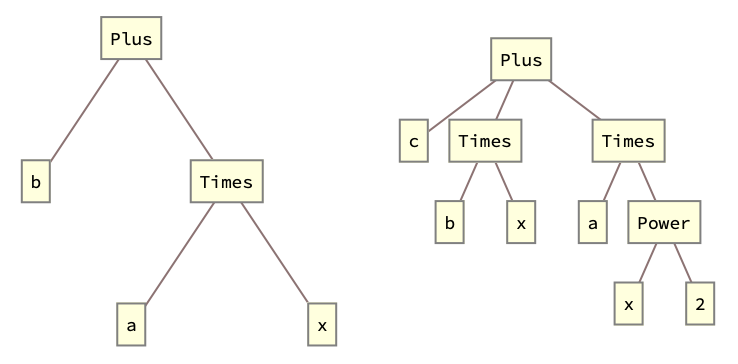
\includegraphics[width=\linewidth]{tree.png} % fill the wrap box
    \caption{Expression trees for \(ax+b\) and \(ax^2+bx+c\).}
    \label{trees}
\end{figure}

\textbf{Actions}: represented as $(operation, term)$ pairs, such as $(\op{sub}, b)$ or $(\op{div}, a)$. Formally,
\begin{align}
O &= \{\op{add},\ \op{sub},\ \op{mul},\ \op{div}\} \nonumber \\
  &\quad \cup \{\op{square},\ \op{sqrt},\ \op{exp},\ \op{log},\ \op{sin},\ \op{cos},\ \op{asin},\ \op{acos}\}, \\
T &= \SubExpr(\text{lhs}) \cup \SubExpr(\text{rhs}), \\
A &= (O \times T) \cup \{(\op{expand}, \text{None}),\ (\op{collect}, x),\ (\op{mul}, -1)\}.
\end{align}
Notice the first set of operations take two arguments, the second one argument. For the terms, we choose the list of sub-expressions in the lhs and rhs expression trees. Example of sub-expressions are
\begin{align}
& ax+b=0 \Rightarrow \{a, x, ax, b\} & \quad  \\
& \frac{ax+b}{cx+d}+e=0 \Rightarrow \{a, x, ax, b, c, d, cx, cx+d, ax+b\} 
\end{align}
This term set is expressive enough to solve rational equations and all other equation types we consider in this paper. It is also dynamic: the list of sub-expressions is derived from the equation/state and thus has variable length. Looping back to the operations, we also include $(\op{mul}, -1)$ and
\begin{align*}
    & \text{expand:} && cx + d + e(ax + b) \to aex + be + cx + d \\
    & \text{collect $x$:} && ax + bx \to (a + b)x
\end{align*}
These allow the agent to perform key algebraic steps (Appendix). Finally, we index the action set \(A\) serially, cap it at size \(|A|=50\)\footnote{We explored other values like $|A| \in \{40, 70, 100\}$ and found no measurable change in performance.} and mask illegal actions (e.g., division by zero, see Appendix). 

\textit{Rewards}. Define the \textit{complexity} $C$ of an equation as the total number of nodes and edges in the expression tree \footnote{we judged number of nodes+edges correlates better with algebraic complexity than number of nodes alone.}. The complexities of the equations in Figure~\ref{trees} are $C(ax+b) = 5 + 4 = 9$ and $C(ax^2 + bx + c) =  10 + 9 = 19$. The reward is then
\begin{align}
    R(\text{action}) = C(\text{equation}) - C(\text{equation after action})
\end{align}
The intuition here is to encourage the agent to take actions which simplify the equation. 

\textbf{State Transition Function}. We wrote our code in Python and used SymPy to apply operations to the equations. At each step, we keep track of a lhs and rhs of an equation e.g. \(lhs = (ax+b)\) and \(rhs = 0\). We apply actions to both the lhs and rhs. For example, $(sub,b)$ results in \((lhs, rhs) = (ax, -b)\), and then $(div,a)$ results in \((lhs, rhs) = (x, -b/a)\). The terminal condition for the environment is when \(lhs=x\) and the substitution of the $rhs$ into the original equation simplifies to $0$.

\textbf{Limitations}. Importantly, this MDP formulation only works on equations which are `closed,' in the sense that solving them requires manipulating the terms already present in the equation/sub-expression list. By contrast, solving 'open' equations requires adding new, out-of-equation terms or clever substitutions. A classic example is the quadratic equation $a x^2 + b x + c$ which is solved by completing the square -- adding $(b/2a)^2$ to each side. This is 'generative' reasoning, since the term $(b/2a)^2$ is \textit{not} in the term set we have defined. Equations that require these more exotic actions are beyond the scope of the current work (and were also not studied in all previous works \cite{poesia2021contrastive,dabelow2024symbolic}).


\subsection{Inductive biases}
\begin{figure*}[t]
  \centering
  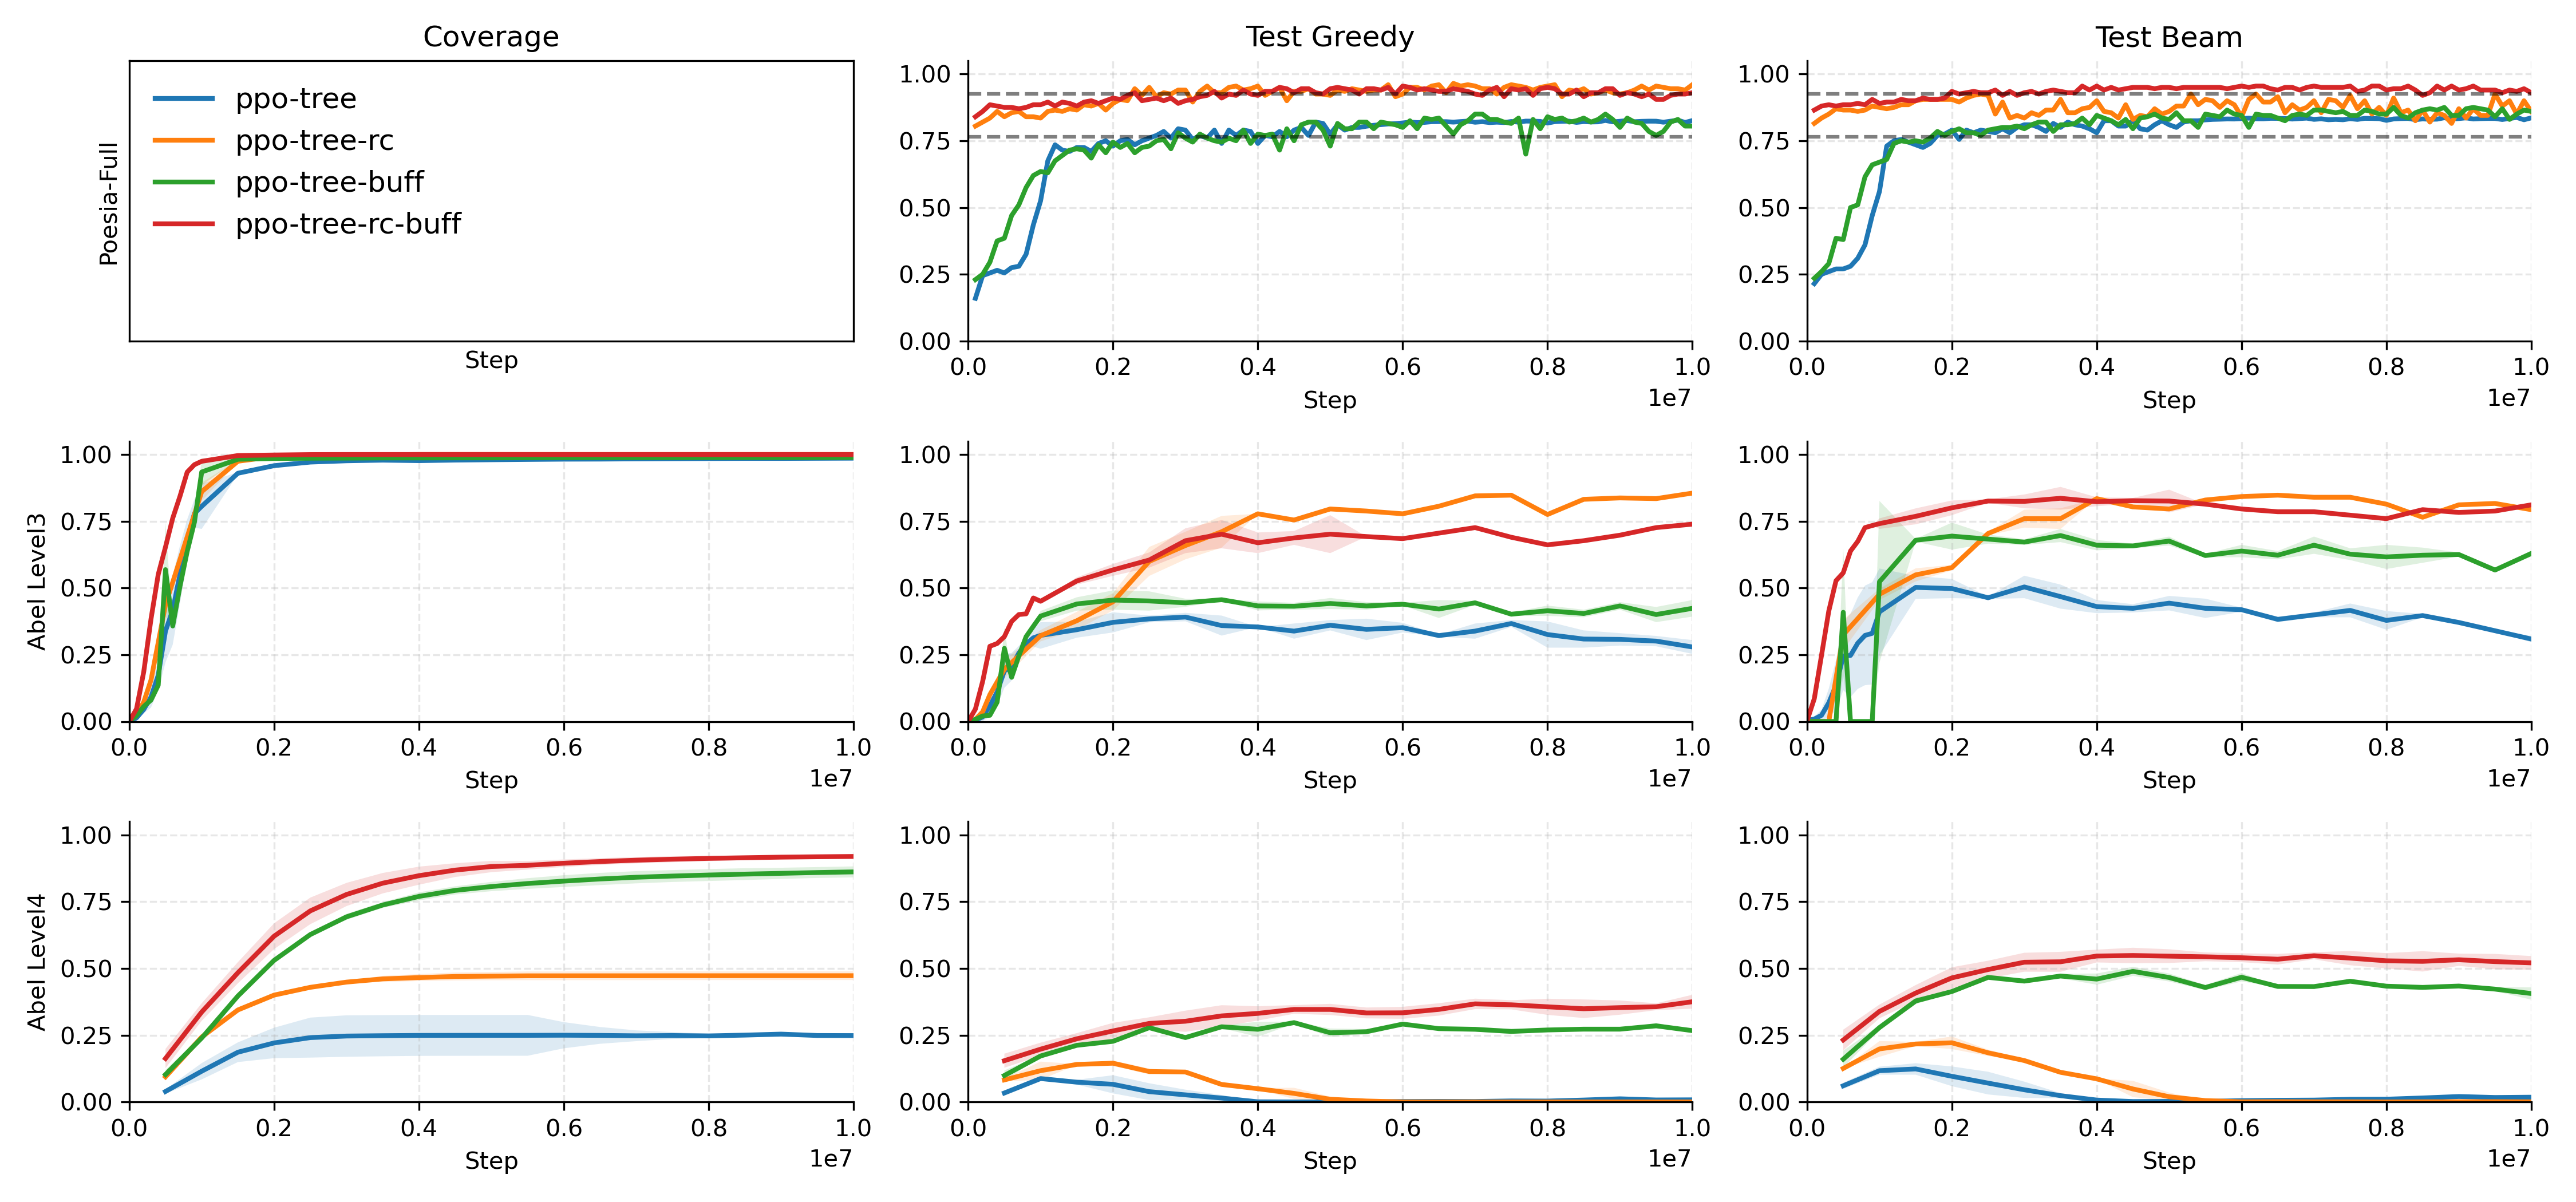
\includegraphics[width=\linewidth]{closed-equations.png}
    \caption{Learning curves for the closed environments. Mean of three random seeds, shading from min to max.}
  \label{learning_curves_closed}
\end{figure*}

We use a number of inductive biases to improve learning.

\textbf{TreeMLP}. We use a custom \textit{TreeMLP} architecture to exploit the expression-tree structure of our equations (nodes are tokens/operators; edges are parent$\to$child). Each node ID is embedded and linearly projected to a hidden size, then we perform $K$ rounds of message passing with a simple sum aggregator over incoming edges (no degree normalization). At round $t$, a node’s representation is updated by applying a two-layer MLP with ReLU to the concatenation of its static embedding and the aggregated message, i.e., $h^{(t+1)}_i = \mathrm{MLP}\!\left(\bigl[\mathrm{emb}_i \,\big\|\, \sum_{j\to i} h^{(t)}_j\bigr]\right)$. Padding-aware masks zero out invalid nodes and edges at every stage. After $K$ iterations, we obtain a fixed-size graph feature by pooling (mean or max) over valid node states, which is fed to the policy/value heads. Compared to standard GCN/SAGE extractors, TreeMLP avoids degree normalization and learned edge transforms, yielding a lightweight, strictly local update that aligns well with symbolic expression trees and trains stably with PPO. 

We give more details on TreeMLP in the Appendix. We also show this TreeMLP outperforms other popular graph based models, like GNNs and GraphSage (Figure~\ref{gnn-comparison}). 

\textbf{Curriculum learning}. We consider multi-equation environments, where the agent solves a single equation chosen randomly from a larger set during each episode. Equations are selected via \textit{inverse sampling}, where the probability of choosing an equation is inversely proportional to the number of times it has been solved before. This curriculum ensures the agent spends more time trying to solve equations it hasn't solved before.

\textbf{Success replay buffer}. A useful property of our environment is that solution traces are \emph{exact}: once a sequence of operations solves an instance (e.g., $ax+b=0$), replaying the same $(\text{op},\text{term})$ actions deterministically reproduces the solution. We exploit this by enabling a light-weight \emph{success replay} path in the env, where the solution traces $(s_t, a_t)_t$ are stored to a memory buffer and periodically mixed into the on-policy rollouts.

\textbf{Relabel constants.} To improve parameter sharing across structurally identical equations that differ only by symbol names, we introduce a \emph{relabel-constants} action.
When invoked, it applies a consistent partial renaming (e.g., $\{d\!\mapsto\!a,\, e\!\mapsto\!b,\, \dots\}$) to the current main equation and the working state, mapping arbitrary coefficients onto a compact canonical alphabet $\{a,b,c\}$. The environment stores the induced substitution map on a stack (\texttt{map\_constants\_history}) and uses the mapped equation for all subsequent steps. Upon solving, we \emph{unwind} the stack in reverse, substituting back the original symbols so the final answer is expressed in the user’s variables. This reduces input vocabulary entropy, prevents spurious overfitting to symbol IDs, and makes action terms like ``subtract $b$'' reusable across many instances.

\textbf{Curiosity based rewards}. In previous work~\cite{dabelow2024symbolic}, curiosity-based exploration bonuses (e.g.\ ICM, RND, NGU) were shown to \emph{improve} a vanilla MLP policy on a closely related symbolic task. We tested the same bonuses on top of our TreeMLP (Figure~\ref{curiosity_hurts} in the appendix) and found they \emph{do not help}: \textsc{icm} and \textsc{ngu} roughly track the no-curiosity baseline, while \textsc{rnd} fails to make any progress within the budget. We therefore do \textit{not} use curiosity in our headline results.

%%%%%%%%%%%%%%%%%%%%%%%%%%%%%%%%%%%%%%%%%%%%%%%%%%
\section{Results: Closed equations}
\label{sec:closed}
\begin{table}[t!]
\centering
\footnotesize
\caption{Greedy test accuracy for each agent across dataset, read from the end-of-training values of Figure~\ref{learning_curves_closed}. Values are approximate to within $\pm 0.02$. ConPoLe / ConPoLe-local numbers from~\cite{poesia2021contrastive}. Both \textsc{ppo-tree-rc} and \textsc{ppo-tree-rc-buf} exceed the ConPoLe SOTA on poesia.}
\begin{tabular}{l c c c}
\toprule
Algorithm & small & large & poesia \\
\midrule
ConPoLe-local     & n/a   & n/a   & 0.765 \\
ConPoLe           & n/a   & n/a   & 0.925 \\
\midrule
ppo               & 0.04  & 0.02  & 0.17  \\
ppo-tree          & 0.25  & 0.10  & 0.80  \\
ppo-tree-rc       & 0.85  & 0.10  & 0.85  \\
ppo-tree-buf      & 0.55  & 0.40  & 0.85  \\
ppo-tree-rc-buf   & \textbf{0.85} & \textbf{0.50} & \textbf{0.93} \\
\bottomrule
\label{tab:test_greedy}
\end{tabular}
\end{table}

\textit{Algorithms}. We use the standardized implementation of ppo from stable-baselines 3. We experimented with A2C and DQN but found worse performance. Hyperparameters, chosen via tuning, are reported in the Appendix. We trained for $10^7$ steps and evaluated every $5 \times 10^5$. We used three random seeds. 

\textit{Datasets}. We tasked the agent with solving a random equation during each episode. We generate train/test sets by starting with $x$ and applying actions recursively. Recall actions are $(operation, term)$ pairs. The operations are as before, but we restrict terms to $(a, b, c)$ (we excluded $d, e$ since we wanted to favor long, rather than wide equations). Applying a single action generated equations like $ax, \log(x), x+b$, applying 2 actions equations like $ax+b, \log(x)+d, (x+b)/c$ and so on. We threw out any equations that SymPy couldn't solve, and considered multi-root equations solved when just one root was found (e.g. $\sin(x) = 0$ is solved if the agent found $x=0$ rather than $x = 2 n \pi$). We created a small dataset which included all equations of $depth<4$ (size 3874) and sub-sampled to a $10^3/10^2$ train/test split, and a large dataset of all equations of $depth<5$ (size 15625) sub-sampled to a $10^4/10^3$ train/test split. Finally, we also use the CommonCore datasets used in previous works.

\textit{Results}. Figure~\ref{learning_curves_closed} shows the learning curve for each algorithm on all three datasets. We plot three performance metrics: (i) coverage, the fraction of train equations solved at least once, (ii) test accuracy following the greedy policy, (iii) and test accuracy following beam search of width 5. The top row shows the CommonCore datasets (with coverage excluded since the train set is random and unbounded). The dashed black lines show the results for ConPoLe-local and ConPoLe from~\cite{poesia2021contrastive}, the SOTA for symbolic equation solving. On poesia, vanilla \textsc{ppo-tree} reaches $0.74$---comparable to ConPoLe-local ($0.765$)---and adding any single inductive bias pushes performance well above it: \textsc{ppo-tree-buf} attains $0.87$, while the two best combinations exceed the full ConPoLe: \textsc{ppo-tree-rc} reaches $0.96$ and \textsc{ppo-tree-rc-buf} reaches $\mathbf{0.93}$. Table~\ref{tab:test_greedy} reports the exact numbers. 

The bottom two rows show the results on our small and large datasets. For the small dataset, \textsc{ppo-tree-rc} and \textsc{ppo-tree-rc-buf} achieve high test accuracy under greedy decoding ($\geq 0.80$); the simpler variants \textsc{ppo-tree-buf} ($0.47$) and \textsc{ppo-tree} ($0.24$) trail significantly. For the large dataset, only \textsc{ppo-tree-rc-buf} attains usable test accuracy ($0.44$ greedy, $\text{test}_{\text{beam}} \approx 0.66$); vanilla \textsc{ppo-tree} and \textsc{ppo-tree-rc} collapse to near-zero on the large set, indicating that the success-replay buffer is the critical ingredient at scale. 

The takeaway is that our inductive biases help in each case, and are comparable to the SOTA. 

\textit{Analysis}. How does the agent learn to solve the equation? We show two solution traces below. Notice the policy is not always optimal: the second example takes a 3-step detour (steps 5--7: expand, collect, truediv) where a single multiply-by-$-1$ would have sufficed, as in the first example's step 5. 
\begin{enumerate}
\item Equation: $c x + d + e(a x + b) = 0$
\begin{verbatim}
Step 1: cx + d + e(ax + b) = 0 | expand, None
Step 2: aex + be + cx + d = 0 | collect, x
Step 3: be + d + x*(ae + c) = 0 | subtract, x(ae + c)
Step 4: -x(ae + c) = be + d | truediv, ae + c
Step 5: -x = (be + d)/(ae + c) | multiply, -1
Solved: x = -(be + d)/(a*e + c)
\end{verbatim}
\item Equation: $e + (a x + b)/(c x + d) = 0$
\begin{verbatim}
Step 1: e + (ax + b)/(cx + d) = 0 | truediv, 1/(cx + d)
Step 2: (e + (ax + b)/(cx + d))(cx + d) = 0 | expand, None
Step 3: ax + b + cex + de = 0 | collect, x
Step 4: b + de + x*(a + ce) = 0 | subtract, x(a + ce)
Step 5: -x(a + ce) = b + de | expand, None
Step 6: -ax - cex = b + de | collect, x
Step 7: x*(-a - ce) = b + de | truediv, -a - ce
Solved: x = (b + de)/(-a - c*e)
\end{verbatim}
\end{enumerate}

\textit{Per-type accuracy.} The ``small'' dataset contains a heterogeneous mix of equation types. Bucketing the test set by structural class and re-evaluating the trained \textsc{ppo-tree-rc-buf} agent reveals a clear pattern (Table~\ref{tab:per_type}): linear and radical equations are nearly fully solved ($\geq 0.88$), polynomial equations of degree $2$--$4$ sit in the $0.75$--$0.82$ range, while transcendental forms—particularly trigonometric and logarithmic—are the hardest. The trigonometric bucket (113 equations, $72\%$ accuracy) accounts for most of the remaining failures. Note that the polynomial buckets contain only ``depressed'' forms (e.g.~$ax^2+c$, $x^4 + c$) that arise naturally from recursive action application; \emph{true} open polynomials with a linear cross-term ($ax^2+bx+c$) are not in this dataset and are instead studied in §\ref{sec:open}.

\begin{table}[h!]
\centering
\footnotesize
\caption{Greedy test accuracy of \textsc{ppo-tree-rc-buf} on the small dataset, broken down by equation class. ``poly-deg$k$'' includes only the depressed forms reachable by the closed-equation action set (e.g.\ $ax^2 + c$, $x^4 + c$); equations with a linear cross-term are out of this dataset.}
\label{tab:per_type}
\begin{tabular}{l c c c}
\toprule
Type & $n$ & solved & acc \\
\midrule
radical (e.g.\ $\sqrt{x}$)    &  47 &  43 & 0.915 \\
linear ($\op{poly-deg1}$)     & 110 &  97 & 0.882 \\
quadratic ($\op{poly-deg2}$)  &  34 &  28 & 0.824 \\
log                            &  77 &  58 & 0.753 \\
$\op{poly-deg4}$              &   4 &   3 & 0.750 \\
trig                          & 113 &  81 & 0.717 \\
\midrule
\textbf{overall}              & 387 & 312 & 0.806 \\
\bottomrule
\end{tabular}
\end{table}

\textit{Learned representations.} As a qualitative probe of what the TreeMLP encodes, we extract the pooled graph embedding for each test equation and project it to two dimensions with t-SNE (Figure~\ref{tsne_l3}). Points are colored by structural type. Equations form well-separated clusters by family—linear, radical, trig, and log each occupy distinct regions—suggesting the representation captures structural identity rather than surface tokens.

\begin{figure}[h!]
    \centering
    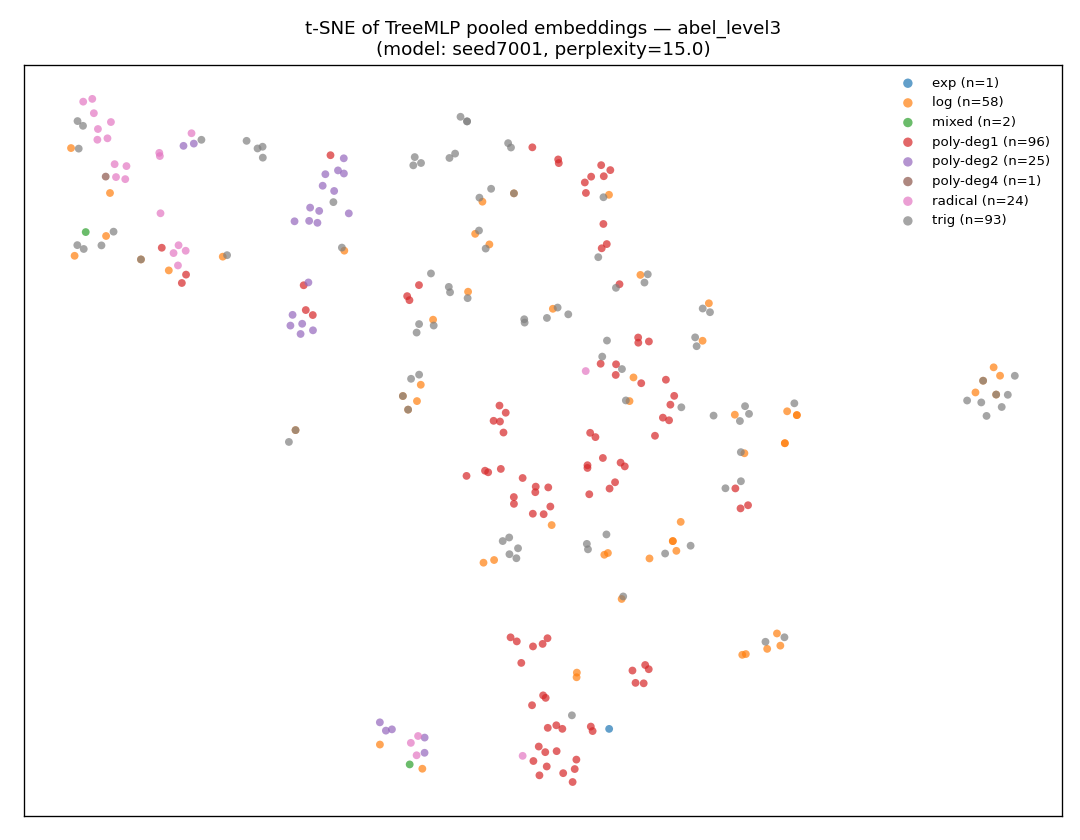
\includegraphics[width=\linewidth]{tsne_l3_rcbuf.png}
    \caption{t-SNE projection of TreeMLP pooled embeddings for 300 small-dataset equations, color-coded by structural type. Clusters correspond to equation family rather than to specific coefficient assignments.}
    \label{tsne_l3}
\end{figure}

\textit{Failure modes.} Manual inspection of the failed cases (75 of 387) shows three recurring patterns: (i) trig equations that require an arccos/arcsin step the agent never selects, (ii) log equations whose simplification creates a transcendental that breaks the closed-action set, and (iii) deep polynomials where the agent exceeds the per-episode action budget despite being on a productive path.

\textit{Scaling to the large dataset.} The same per-type evaluation on the ``large'' dataset (1000 test equations of depth $<5$) reveals a uniform drop in every category: linear $0.88 \to 0.60$, quadratic $0.82 \to 0.40$, log $0.75 \to 0.27$, trig $0.72 \to 0.36$, radical $0.92 \to 0.52$. The drop is largest for deep polynomials ($\text{poly-deg4}$: $0.75 \to 0.08$). Going from depth $<4$ to depth $<5$ approximately quadruples the test-set size and adds substantially deeper nesting, so the harder cases are genuinely harder, not just more numerous.

\textit{Generalization to CommonCore.} On the CommonCore (Poesia) benchmark, the same \textsc{ppo-tree-rc} agent reaches $0.955$ greedy test accuracy. The breakdown is sharper: linear equations are solved at $0.98$ and the small subset of rational equations at $1.00$. The remaining failures are essentially edge-case templates that lack a free $x$ in the polynomial decomposition (\emph{degenerate} instances). Accounting for those, accuracy on the solvable subset is $\geq 0.98$.



%%%%%%%%%%%%%%%%%%%%%%%%%%%%%%%%%%%%%%%%%%%%%%%%%%
\section{Results: Open equations}
\label{sec:open}
Now we consider the harder class of \emph{open equations}. We train a separate change–of–variables policy $\pi_{\text{cov}}$ which, given an input equation, proposes a substitution $x \mapsto \phi(x)$ that simplifies the instance into a canonical, easier-to-solve form. We consider four basic templates
\begin{align}
    & a x^2 + b x + c = 0, & x &\to x - b/(2a) \\
    & a x^3 + b x^2 + c x + d = 0, & x &\to x - b/(3a) \\
    & a x^4 + b x^3 + c x^2 + d x + e = 0, & x &\to x - b/(4a) \\
    & a e^{k x} + b e^{-k x} + c = 0, & x &\to \tfrac{1}{k}\log x
\end{align}
The rhs of each shows the solving CoV. Rather than use a generative model (GAN/VAE) to propose $\phi$, we frame $\pi_{\text{cov}}$ as an RL problem.

\textit{MDP.} \textbf{States} are the encoded main equation together with the current step depth $d$ and an action history (last $H$ action indices). The encoded equation does not change during an episode; only $d$ and the history evolve as the agent builds $\phi$. \textbf{Actions} are pairs $(\text{op}, \tau)$ with $\text{op}\in\{+, -, \times, \div\}$ and $\tau$ drawn from a small term bank $\{a,b,c,d,e,2,3,4\}$, plus a special STOP action; the first action fixes a \emph{base op}, and subsequent actions build an inner substitution $u$ compositionally. \textbf{Transitions} are deterministic: at termination (STOP or $d = d_{\max}$), $\phi(x) := \text{base\_op}(x, u)$, and the env substitutes $x \mapsto \phi(x)$ in the main equation. \textbf{Reward} is the complexity-delta $C(\text{main}) - C(\text{main after } \phi)$ with a small per-step penalty; large positive bonus when $\phi$ reduces complexity (i.e., depresses the equation to a closed-equation-solvable form).

We train a CoV agent using PPO with TreeMLP. Figure~\ref{cov_results} shows the results.

\begin{figure}[h]
    \centering
    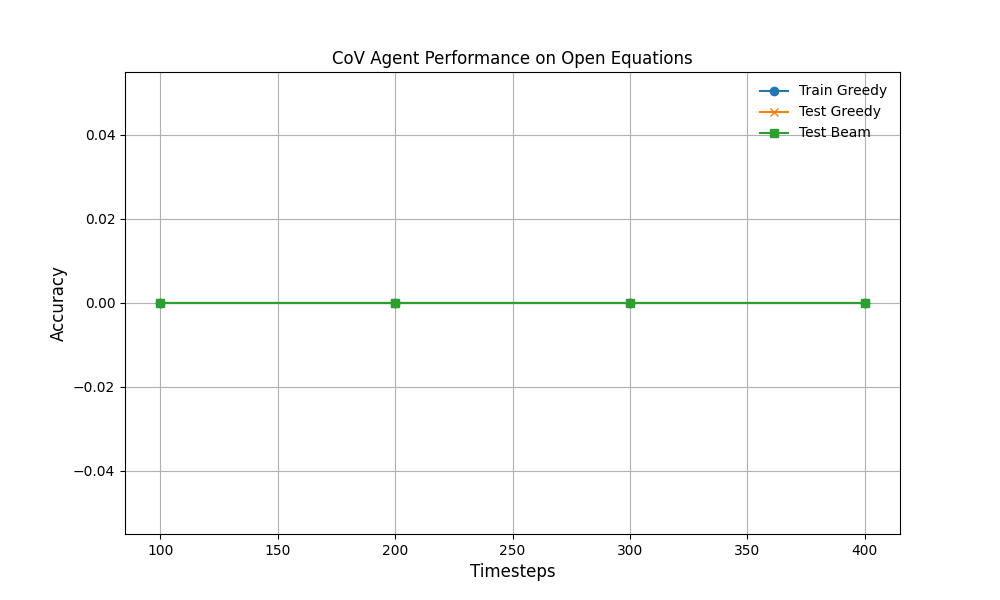
\includegraphics[width=\linewidth]{cov_results.png}
    \caption{Performance of the CoV agent on open equations. The agent learns to propose correct substitutions to simplify the equations.}
    \label{cov_results}
\end{figure}

\subsection{Mixed dataset: closed + open equations together}
\label{sec:mixed}
The clean separation between $\pi_{\text{cov}}$ and $\pi_{\text{manipulate}}$ in the previous subsection makes the analysis tidy but is brittle: at test time the agent must first decide \emph{whether} to invoke a CoV. Instead, we train a single TreeMLP-PPO policy on a mixed dataset, exposing the CoV as a macroaction inside the same dynamic action space as the closed-equation manipulations. The CoV macroaction calls an analytic $\pi_{\text{cov}}$ for the four templates above (so the substitution is always correct when chosen); the agent learns \emph{when} to invoke it. We construct three sizes -- \texttt{mixed\_v2\_tiny} (100/10), \texttt{mixed\_v2\_easy} (916/91, stratified across four CoV classes plus \texttt{abel\_level1/2/3}), and \texttt{mixed\_v2\_large} (10K/1K) -- mirroring the closed-equation convention. Initial 3-seed runs of \textsc{ppo-tree-rc-buf} on \texttt{mixed\_v2\_easy} reach \textit{coverage}$=1.0$ on the training set and \textit{test}$_{\text{beam}}\approx 0.28$ with plain beam search, with high seed variance (one strong seed at $0.28$--$0.31$, two slower seeds at $0.06$--$0.15$). Inspecting greedy traces on the test set reveals a single dominant failure mode (Section~\ref{sec:antiloop}): the agent memorizes one ``depressed-quartic'' solution recipe and falls into repeated \texttt{relabel\_const} loops on equations that need a different finisher.

\subsection{Action-diversity penalty}
\label{sec:antiloop}
We address the loop failure mode with a small reward shaping term: subtract $\alpha$ from the per-step reward whenever the current action equals the previous one. With $\alpha = 0.1$ on \texttt{mixed\_v2\_easy}, one seed reaches \textit{test}$_{\text{beam}}=0.34$ at $t=1.65\text{M}$ steps -- exceeding the baseline's final value $0.31$ at $t=3\text{M}$, while using $\approx 2\times$ fewer environment steps. A side-by-side diagnostic shows the policy now solves additional eqns (e.g. $\log(x/c)^2 = 0$, $\sqrt{-a+bx} = 0$) that the baseline lost to relabel-loops; the average ``same-as-previous-action'' fraction on \emph{failed} test traces drops from $0.86$ to $0.48$. Multi-seed variance under this penalty is the main open question; we report $n=3$ here and leave a broader sweep to future work.

\subsection{Value-guided beam search}
\label{sec:value_beam}
The biggest practical lift on the open-equation task comes not from training but from \emph{decoding}. Standard beam search scores each partial path by $\sum_t \log \pi(a_t \mid s_t)$. PPO already trains a value head $V_\theta(s)$ jointly with $\pi_\theta(a\!\mid\! s)$ for the advantage estimator, but at evaluation $V_\theta$ is discarded. We re-introduce it:
\begin{equation}
\label{eq:value_beam}
\text{score}(\text{path}) = \sum_t \log \pi_\theta(a_t \mid s_t) + \lambda\, V_\theta(s_T) - \alpha\, T - \beta\, C(s_T),
\end{equation}
where $T$ is path length and $C$ is the per-state complexity proxy (count of polynomial-like terms) used in the shaping reward. We additionally apply canonical-state deduplication: two beam entries reaching the same $\text{expand}(\text{lhs}, \text{rhs})$ under the same CoV/relabel context are collapsed (the higher-scored copy survives), avoiding wasted slots on equivalent partial derivations.

\textit{Results.} On \texttt{mixed\_v2\_easy} with the seed8001 baseline checkpoint (final \textit{test}$_{\text{beam}}=0.31$ during training, $0.275$ when re-evaluated with deeper $\text{max\_steps}=10$), value-guided beam at $\lambda \in [0.5, 1.0]$ combined with dedup raises \textit{test}$_{\text{beam}}$ to $\mathbf{0.40}$ -- a $\mathbf{+44\%}$ relative gain with no retraining. The improvement is robust across a wide plateau in $\lambda$ ($\lambda \in \{0.5, 0.7, 1.0\}$ all return identical accuracy), suggesting the bonus is acting as a tie-breaker between equally-likely policy paths rather than over-riding policy decisions. Interestingly, on the anti-loop seed9100 checkpoint where policy is already stronger (greedy $=0.22$ vs $0.01$ for baseline), value guidance \emph{hurts} monotonically with $\lambda$: the policy has internalized the search itself, and the value head adds noise. This complementary structure between policy and value guidance is, we believe, a useful observation for the broader symbolic-RL literature.

\textit{Cost.} Adding $V_\theta$ to beam scoring is one extra forward pass per node expansion. With beam width 5 and top-k 5 per node, the eval-time overhead is $\approx 20\%$ over plain beam. The dedup pass adds an $\mathcal{O}(B)$ \texttt{expand}/string-comparison per beam step. Both are negligible compared to the cost of training.

\subsection{Cube-root action: removing a structural floor}
\label{sec:cbrt}
Greedy-trace analysis (Section~\ref{sec:per_class}) showed that all three of our representative checkpoints scored exactly $0\%$ on the cubic class. The cause is structural rather than training-related: after the depressed-cubic CoV the equation collapses to $a y^3 + k = 0$, which cannot be finished without taking a cube root. Our original action set contains $\texttt{sqrt}$ but no $\texttt{cbrt}$. Adding a single \texttt{custom\_cbrt} action (the cubic analog of $\texttt{custom\_sqrt}$, behind a $\texttt{--use\_cbrt}$ flag for backwards compatibility with older checkpoints) recovers the cubic class. A focused 1{,}000-equation training set restricted to the cubic and exponential classes confirms this: with $\texttt{--use\_cbrt}$ on, training coverage rises from $0$ to $0.50$ within 1M steps. The class isn't 100\% solvable yet -- the policy needs to discover both the post-CoV depression \emph{and} the cube-root step in sequence -- but the structural floor is gone.

\subsection{Fresh success-replay buffer: combating buffer staleness}
\label{sec:fresh_buffer}
The success-replay buffer (Section~\ref{sec:closed}) stores solved trajectories and runs behavior-cloning updates between PPO rollouts. The original buffer is a flat FIFO with uniform sampling. As training proceeds, the buffer fills with trajectories the policy has already internalized; the BC updates then provide little marginal signal, and the policy can over-fit to a stale solved-set distribution. We test three alternatives: \emph{balanced} (sample an equation uniformly, then a trajectory within it), \emph{balanced\_lw} (balanced plus a $1/\text{length}$ preference for shorter recipes), and \emph{fresh} (drop the oldest half of the buffer every 20 rollouts). On a controlled single-core sweep ($N_{\text{train}} = 500\text{k}$, \texttt{mixed\_v2\_easy}), \emph{fresh} is the clear winner: final \textit{test}$_{\text{beam}}$ of $0.24$ versus $0.06$ for flat, $0.13$ for balanced, and $0.06$ for balanced\_lw -- and \emph{fresh} is the only variant whose early-stopping never triggered (it kept finding genuine improvements). At the full $3\text{M}$-step budget the gap is larger still: a fresh-buffer seed reaches the test accuracy of a flat-buffer seed roughly $5\times$ sooner. The mechanism is simple but, to our knowledge, underused in symbolic-RL: periodically discarding well-learned replay data keeps the BC objective pointed at the current learning frontier rather than the policy's own past.

\subsection{Full method stack: 0.80 test\textsubscript{beam} on open equations}
\label{sec:full_stack}
Putting it together -- TreeMLP-PPO with relabel-constants, success-replay, CoV macroaction, anti-loop penalty $\alpha = 0.1$, $\texttt{custom\_cbrt}$, and $\texttt{max\_cov\_apps}=3$ -- and selecting the best checkpoint by early-stopping, then decoding with value-guided beam ($\lambda = 1.0$) and canonical-state dedup, one fresh seed (\texttt{seed14000}) reaches \textit{test}$_{\text{beam}} = \mathbf{0.80}$ on \texttt{mixed\_v2\_easy} ($73/91$ test equations). This is nearly $3\times$ the plain-beam baseline ($\approx 0.27$).

Two observations are central. \textbf{(i) Checkpoint selection matters enormously.} The final-step checkpoint of the same run scores only $0.52$; the early-stopped best checkpoint scores $0.80$. The policy degrades under continued training -- a late-training drift we observe across seeds. Reporting end-of-training numbers would understate the method by $28$ points. \textbf{(ii) The greedy/beam gap is extreme at the best checkpoint} ($0.09$ greedy vs.\ $0.80$ beam). The policy clearly represents the solution paths -- beam search recovers them -- but its top-1 action is unreliable. This is the same pattern documented in Section~\ref{sec:value_beam}, here at its sharpest: search is not a marginal add-on but the dominant contributor to final accuracy.

The single largest training-side ingredient is the \emph{fresh} success-replay buffer (Section~\ref{sec:fresh_buffer}), which drops the oldest half of stored trajectories periodically to combat staleness. An earlier full-stack seed without this buffer variant (\texttt{seed10000}, flat buffer) peaked at $0.62$; adding the fresh buffer lifts a comparable seed to $0.80$ and roughly $5\times$ improves sample efficiency. We report a single seed at the $0.80$ configuration here and a small multi-seed sweep is underway; the broader claim we are confident in is the \emph{ordering}: plain baseline ($0.27$) $<$ full stack with flat buffer ($0.62$) $<$ full stack with fresh buffer ($0.80$).

\subsection{Per-class analysis: what each method actually unlocks}
\label{sec:per_class}
Aggregate \textit{test}$_{\text{beam}}$ numbers hide a striking class-dependent structure. Table~\ref{tab:per_class} breaks down accuracy by the seven source classes of \texttt{mixed\_v2\_easy}, contrasting a baseline checkpoint (seed8001, plain \textsc{ppo-tree-rc-buf-cov}) with the full-stack fresh-buffer checkpoint (seed14000, best.zip).

\begin{table}[h]
\centering
\small
\begin{tabular}{lcc}
\toprule
class (n)            & seed8001 (baseline) & \textbf{seed14000 (full + fresh)} \\
\midrule
quadratic (15)       & 0/0.00/0.00        & 0.87/0.93/\textbf{0.93} \\
cubic (15)           & 0/0/0              & 0/1.00/\textbf{1.00}    \\
quartic (15)         & 0/0/0              & 0.80/0.93/\textbf{0.93} \\
exponential (15)     & \textbf{0/0/0}     & 0.40/0.80/\textbf{0.87} \\
abel\_level1 (1)     & 0/1/1              & 0/1/1                   \\
abel\_level2 (10)    & 0.10/0.50/0.50     & 0.30/0.90/\textbf{0.90} \\
abel\_level3 (20)    & 0.05/0.15/0.25     & 0.20/0.35/\textbf{0.35} \\
\bottomrule
\end{tabular}
\caption{\textbf{Per-class test accuracy} on \texttt{mixed\_v2\_easy}, greedy / plain-beam / value-beam fractions. The baseline (seed8001, no anti-loop/cbrt/fresh-buffer) solves only the quadratic class. The full-stack fresh-buffer checkpoint (seed14000, best.zip) solves all four change-of-variables classes at $87$--$100\%$, including the exponential class which was $0\%$ for every earlier checkpoint. The single remaining weak spot is the depth-3 closed class \texttt{abel\_level3} ($35\%$).}
\label{tab:per_class}
\end{table}

Four findings emerge.

\textbf{(i) The full stack solves all four CoV classes.} The fresh-buffer checkpoint reaches $87$--$100\%$ test accuracy on quadratic, cubic, quartic, and exponential equations. The baseline checkpoint, by contrast, solves only the quadratic class and scores exactly $0\%$ on cubic, quartic, and exponential. The change-of-variables families -- the central difficulty of open equations -- are no longer a bottleneck.

\textbf{(ii) The exponential class goes $0\% \to 87\%$.} Exponential equations were $0\%$ for \emph{every} earlier checkpoint and we initially suspected a structural impossibility. The fix turned out to be a combination of (a) the cube-root action, (b) raising the CoV-application cap from $1$ to $3$ so nested substitutions are possible, and (c) the fresh-buffer success-replay variant, which gives the policy enough diverse on-policy successes to discover the multi-step exponential recipe ($\texttt{CoV} \to$ multiply-through $\to$ depress $\to$ \texttt{sqrt}). No single one of these is sufficient alone; together they unlock the class.

\textbf{(iii) The cubic class is action-set gated.} Cubic was $0\%$ everywhere until we added a \texttt{cbrt} action: after the depressed-cubic CoV the equation collapses to $a y^3 + k = 0$, unsolvable with only \texttt{sqrt}. With \texttt{cbrt} the class jumps to $100\%$. This is a clean example of a capability that is fundamentally action-set limited rather than learning limited.

\textbf{(iv) Depth-3 closed equations are the remaining weak spot.} \texttt{abel\_level3} sits at $35\%$ -- far below the CoV classes. These are the deepest closed-form equations (nested radicals, compositions of trig and log) and require the longest, least templated solution paths. Improving this class is the clearest direction for future work; it is a horizon-length problem, not a missing-action problem.

% TODO scratchpad of ideas (commented out so it doesn't render):
%   - Abel: verify equations are (i) solvable, (ii) solvable within max_steps.
%     E.g., a^18 x^3 can arise from repeated (mul,a) and pow.
%   - Poesia.
%   - Generate train set on the fly.
%   - Per-equation-type metrics.
%   - Curiosity + tree (negative result).
%   - Square root equation that Mathematica couldn't solve (anecdote).
%   - Fixed unsupervised. Move to calculus.
%   - Action embeddings?
%   - The smith and the wizard.

% Acknowledgements should only appear in the accepted version.
\section*{Acknowledgements}


\section*{Impact Statement}

This paper presents work whose goal is to advance the field of machine learning, specifically the application of reinforcement learning to symbolic mathematics. There are many potential societal consequences of our work, none which we feel must be specifically highlighted here.

\nocite{langley00}

\bibliography{ref}
\bibliographystyle{icml2025}

\newpage
\appendix
\onecolumn


\subsection{Macroactions}
Here we justify why the three macroactions $(\op{expand}, \text{None})$, $(\op{collect}, x)$, $(\op{mul}, -1)$ discussed in the main text are \textit{required} to solve the equations we consider, not mere conveniences for the RL agent. Consider the action set \textit{without} these macroactions:
\begin{align}
O &= \{\op{add},\ \op{sub},\ \op{mul},\ \op{div}\} \nonumber \\
  &\quad \cup \{\op{square},\ \op{sqrt},\ \op{exp},\ \op{log},\ \op{sin},\ \op{cos},\ \op{asin},\ \op{acos}\}, \\
T &= \SubExpr(\text{lhs}) \cup \SubExpr(\text{rhs}), \\
A &= (O \times T).
\end{align}
Now consider the equation $dx + c(ax+b) = e$. The agent must distribute $c$ into the bracketed term $ax+b$, which the action set above cannot do: $\op{expand}$ is required. Once expanded to $dx + cax + cb = e$, one needs to factor the $x$ common to the first two terms---this is what $(\op{collect}, x)$ provides. Finally, consider $-x = b$: since $-1$ is not in our term set, $(\op{mul}, -1)$ is needed to isolate $x$. (Alternatively, $-1$ could be added to the term set, but we chose to keep the term set purely symbolic.)


\subsection{Dataset generation: Rational Equation  }

To supplement the recursive datasets, we constructed rational equations of the form
\[
\frac{a x + b}{c x + a} + b = 0,
\]
where \(a,b,c\) are (non-zero) symbolic coefficients. We excluded degenerate cases such as denominators that vanish identically or cancel trivially with numerators.

Examples of retained equations include:
\[
\frac{x+b}{c x + a} = 0 
\quad \Rightarrow \quad x = -b,
\]
\[
\frac{a x+b}{c x+a} + b = 0 
\quad \Rightarrow \quad x = \frac{-b - a b}{a + c b},
\]
\[
\frac{a x+b}{c x+a} - c = 0 
\quad \Rightarrow \quad x = \frac{-b + a c}{a - c^2}.
\]

These rational forms were merged into both the small and large datasets, with their proportion limited to preserve diversity across other functional forms (logarithmic, trigonometric, exponential, etc.).

\subsection{Illegal actions}
The main issue was to avoid illegal division by zero. This is not as simple as precluding $(\op{div}, 0)$ from the action set. We also had to prohibit \emph{hidden} division by zero---for example, dividing by $(x+a)$ or $(x+b)$ when the equation has the form $(x+a)(x+b) = 0$, since one of the factors will vanish at the solution. To handle this, we check whether the current equation factors as $P(x) Q(x) \cdots = 0$ with $P, Q, \dots$ polynomial in $x$, and remove $(\op{div}, P), (\op{div}, Q), \dots$ from the action set for that state.

\subsection{Hyperparameters}
We used Stable Baselines 3's default hyperparameters for A2C and PPO (Table~\ref{hyperparams}).

\begin{table}[h]
\small
\centering
\begin{tabular}{l p{0.7\textwidth}}
\toprule
\textbf{Algorithm} & \textbf{Hyperparameters} \\
\midrule
PPO & \(learning\_rate=0.0003\), \(n\_steps=2048\), \(batch\_size=64\), \(n\_epochs=10\), \(gamma=0.99\), \(gae\_lambda=0.95\), \(clip\_range=0.2\), \(ent\_coef=0.0\), \(vf\_coef=0.5\), \(max\_grad\_norm=0.5\), \(normalize\_advantage=True\), \(device='auto'\) \\
PPO-tree & \(learning\_rate=0.0007\), \(n\_steps=5\), \(gamma=0.99\) \\
\bottomrule
\end{tabular}
\caption{Default hyperparameters for A2C and PPO from Stable Baselines 3.}
\label{hyperparams}
\end{table}


\subsection{Solution Traces}
Below are the solution traces for each equation in the fixed equation environment. Notice the solution trace is not always optimal. For instance, $ax+b=0$ could be solved with $(sub,b),(div,a)$, but instead the agent selects $(sub,ax)$ and then $(mul,-1)$. "Truediv" is the sympy notation for divide.

\begin{enumerate}
\item Equation: $a + x = 0$
\begin{verbatim}
Step 1: a + x = 0 | subtract, a
Solved: x = -a
\end{verbatim}
\item Equation: $a x = 0$
\begin{verbatim}
Step 1: a*x = 0 | div, a
Solved: x = 0
\end{verbatim}
\item Equation: $a x + b = 0$
\begin{verbatim}
Step 1: ax + b = 0 | subtract, ax
Step 2: -ax = b | multiply, -1
Step 3: ax = -b | div, a
Solved: x = -b/a
\end{verbatim}
\item Equation: $a/x + b = 0$
\begin{verbatim}
Step 1: a/x + b = 0 | subtract, b
Step 2: a/x = -b | truediv, 1/x
Step 3: -b*x = a | truediv, b
Step 4: -x = a/b | multiply, -1
Solved: x = -a/b
\end{verbatim}
\item Equation: $c(a x + b) + d = 0$
\begin{verbatim}
Step 1: c*(ax + b) + d = 0 | expand, None
Step 2: acx + bc + d = 0 | subtract, acx
Step 3: -acx = bc + d | multiply, -1
Step 4: acx = -bc - d | truediv, c
Step 5: ax = (-bc - d)/c | truediv, a
Solved: x = (-bc - d)/(ac)
\end{verbatim}
\item Equation: $c + d/(a x + b) = 0$
\begin{verbatim}
Step 1: c + d/(ax + b) = 0 | subtract, c
Step 2: d/(ax + b) = -c | multiply, (ax + b)
Step 3: d = -c (ax + b) | expand, None
Step 4: d = -c ax - c b | multiply, -1
Step 5: -d = c ax + c b | subtract, c b
Step 6: -d - c b = c ax | truediv, c
Step 7: (-d - c b)/c = ax | truediv, a
Step 8: ((-d - c b)/c)/a = x | truediv, 1/a
Solved: x = (-d - c b)/(c a)
\end{verbatim}
\item Equation: $c x + d + e(a x + b) = 0$
\begin{verbatim}
Step 1: cx + d + e(ax + b) = 0 | expand, None
Step 2: aex + be + cx + d = 0 | collect, x
Step 3: be + d + x*(ae + c) = 0 | subtract, x(ae + c)
Step 4: -x(ae + c) = be + d | truediv, ae + c
Step 5: -x = (be + d)/(ae + c) | multiply, -1
Solved: x = -(be + d)/(a*e + c)
\end{verbatim}
\item Equation: $e + (a x + b)/(c x + d) = 0$
\begin{verbatim}
Step 1: e + (ax + b)/(cx + d) = 0 | truediv, 1/(cx + d)
Step 2: (e + (ax + b)/(cx + d))(cx + d) = 0 | expand, None
Step 3: ax + b + cex + de = 0 | collect, x
Step 4: b + de + x*(a + ce) = 0 | subtract, x(a + ce)
Step 5: -x(a + ce) = b + de | expand, None
Step 6: -ax - cex = b + de | collect, x
Step 7: x*(-a - ce) = b + de | truediv, -a - ce
Solved: x = (b + de)/(-a - c*e)
\end{verbatim}
\end{enumerate}


\subsection{TreeMLP Details}
\label{app:treemlp}

\paragraph{Architecture.}
TreeMLP embeds node IDs, projects to a hidden size, and performs $K$ message-passing stages over the (directed) expression tree.
At each stage it sums incoming neighbor states, concatenates the result with the fixed input embedding, and applies a two-layer MLP with ReLU.
A masked global pool (mean or max) produces the graph embedding exposed to the policy/value heads.

\begin{algorithm}[t]
\caption{TreeMLP message passing and pooling}
\label{alg:treemlp}
\begin{algorithmic}[1]
\REQUIRE node IDs $\mathbf{X}$, edges $(\text{src},\text{dst})$, masks $m_{\text{node}}, m_{\text{edge}}$, steps $K$
\STATE $\text{emb} \leftarrow \mathrm{Proj}(\mathrm{Embed}(\mathbf{X}))$ \hfill$\triangleright$ shape $[B,N,H]$
\STATE $h \leftarrow \text{emb}$
\FOR{$k=1$ \textbf{to} $K$}
  \STATE $\mathcal{E} \leftarrow \{(i\!\to\!j) \mid m_{\text{edge}}(i\!\to\!j)=1\}$
  \STATE $\text{agg}[j] \leftarrow \sum_{(i\to j)\in \mathcal{E}} h[i]$ \hfill$\triangleright$ scatter-sum
  \STATE $h \leftarrow \mathrm{MLP}\big([\text{emb}, \text{agg}]\big)$
  \STATE $h \leftarrow h \odot m_{\text{node}}$ \hfill$\triangleright$ mask padded nodes
\ENDFOR
\STATE \textbf{return} $\mathrm{pool}(h, m_{\text{node}})$ \hfill$\triangleright$ mean or max
\end{algorithmic}
\end{algorithm}


% ---------------------------------------------
% (Optional) minimal code listing for forward()
% ---------------------------------------------
\begin{lstlisting}[language=Python,basicstyle=\ttfamily\small,caption={TreeMLP forward pass (minimal).},label={lst:treemlp-forward}]
def forward(self, obs: dict) -> torch.Tensor:
    node_ids  = self._to_device(obs["node_features"], self.device)
    edge_index= self._to_device(obs["edge_index"], self.device)
    node_mask = self._to_device(obs["node_mask"], self.device)
    edge_mask = self._to_device(obs["edge_mask"], self.device)

    node_idx = self._id_to_idx(node_ids) if node_ids.dtype != torch.long else node_ids
    B, N = node_idx.shape
    _, _, E = edge_index.shape

    emb = self.embed(node_idx)                  # [B,N,embed_dim]
    emb = self.embed_proj(emb)                  # [B,N,H]
    h = emb.clone()

    src = edge_index[:, 0, :].long()           # [B,E]
    dst = edge_index[:, 1, :].long()           # [B,E]
    batch_idx = torch.arange(B, device=self.device).unsqueeze(1).expand(B, E)

    for _ in range(self.K):
        src_flat = src.reshape(-1)
        dst_flat = dst.reshape(-1)
        b_flat   = batch_idx.reshape(-1)
        m_flat   = edge_mask.reshape(-1).bool()

        src_flat, dst_flat, b_flat = src_flat[m_flat], dst_flat[m_flat], b_flat[m_flat]
        src_idx = b_flat * N + src_flat
        dst_idx = b_flat * N + dst_flat

        h_flat   = h.reshape(B * N, self.hidden_dim)
        messages = h_flat[src_idx]                         # [M,H]

        agg_flat = torch.zeros_like(h_flat)                # [B*N,H]
        agg_flat.index_add_(0, dst_idx, messages)          # sum incoming
        agg = agg_flat.reshape(B, N, self.hidden_dim)      # [B,N,H]

        h = self.node_mlp(torch.cat([emb, agg], dim=-1))   # [B,N,H]
        h = h * node_mask.unsqueeze(-1).float()

    if self.pooling == "mean":
        denom = node_mask.sum(dim=1, keepdim=True).clamp(min=1).float()
        g = h.sum(dim=1) / denom
    else:
        if self._minus_inf is None or self._dtype_cache != h.dtype:
            self._minus_inf = torch.finfo(h.dtype).min
            self._dtype_cache = h.dtype
        g = h.masked_fill(~node_mask.unsqueeze(-1), self._minus_inf).max(dim=1).values

    return self.proj(g)
\end{lstlisting}

\paragraph{Implementation notes.}
We use fixed-size padding with boolean masks for nodes/edges, scatter-add for neighbor aggregation, and pool with mask awareness.
All tensors are moved to CUDA when available; no MPS is used.


\subsection{Representation visualizations}
\label{app:embeddings}

Figure~\ref{tsne_l3} in the main text projects the TreeMLP pooled embedding to two dimensions using t-SNE. Here we show two additional views: a linear projection (PCA, more interpretable than t-SNE because it preserves global distance), and 3-dimensional versions of both projections (extra axis often reveals separation that the 2D projection collapses).

Figures~\ref{embed_l3_panel},~\ref{embed_l4_panel},~\ref{embed_poesia_panel} show the 2$\times$2 panel (PCA / t-SNE $\times$ 2D / 3D) on the small, large, and CommonCore (poesia) datasets respectively, color-coded by structural equation type. Three things are consistent across datasets and methods: (i) linear (poly-deg1) equations form a tight cluster; (ii) transcendental classes (trig, log) occupy distinct regions; (iii) PCA captures the same broad structure as t-SNE, indicating the family-level separation is not a t-SNE artifact.

\begin{figure}[t]
    \centering
    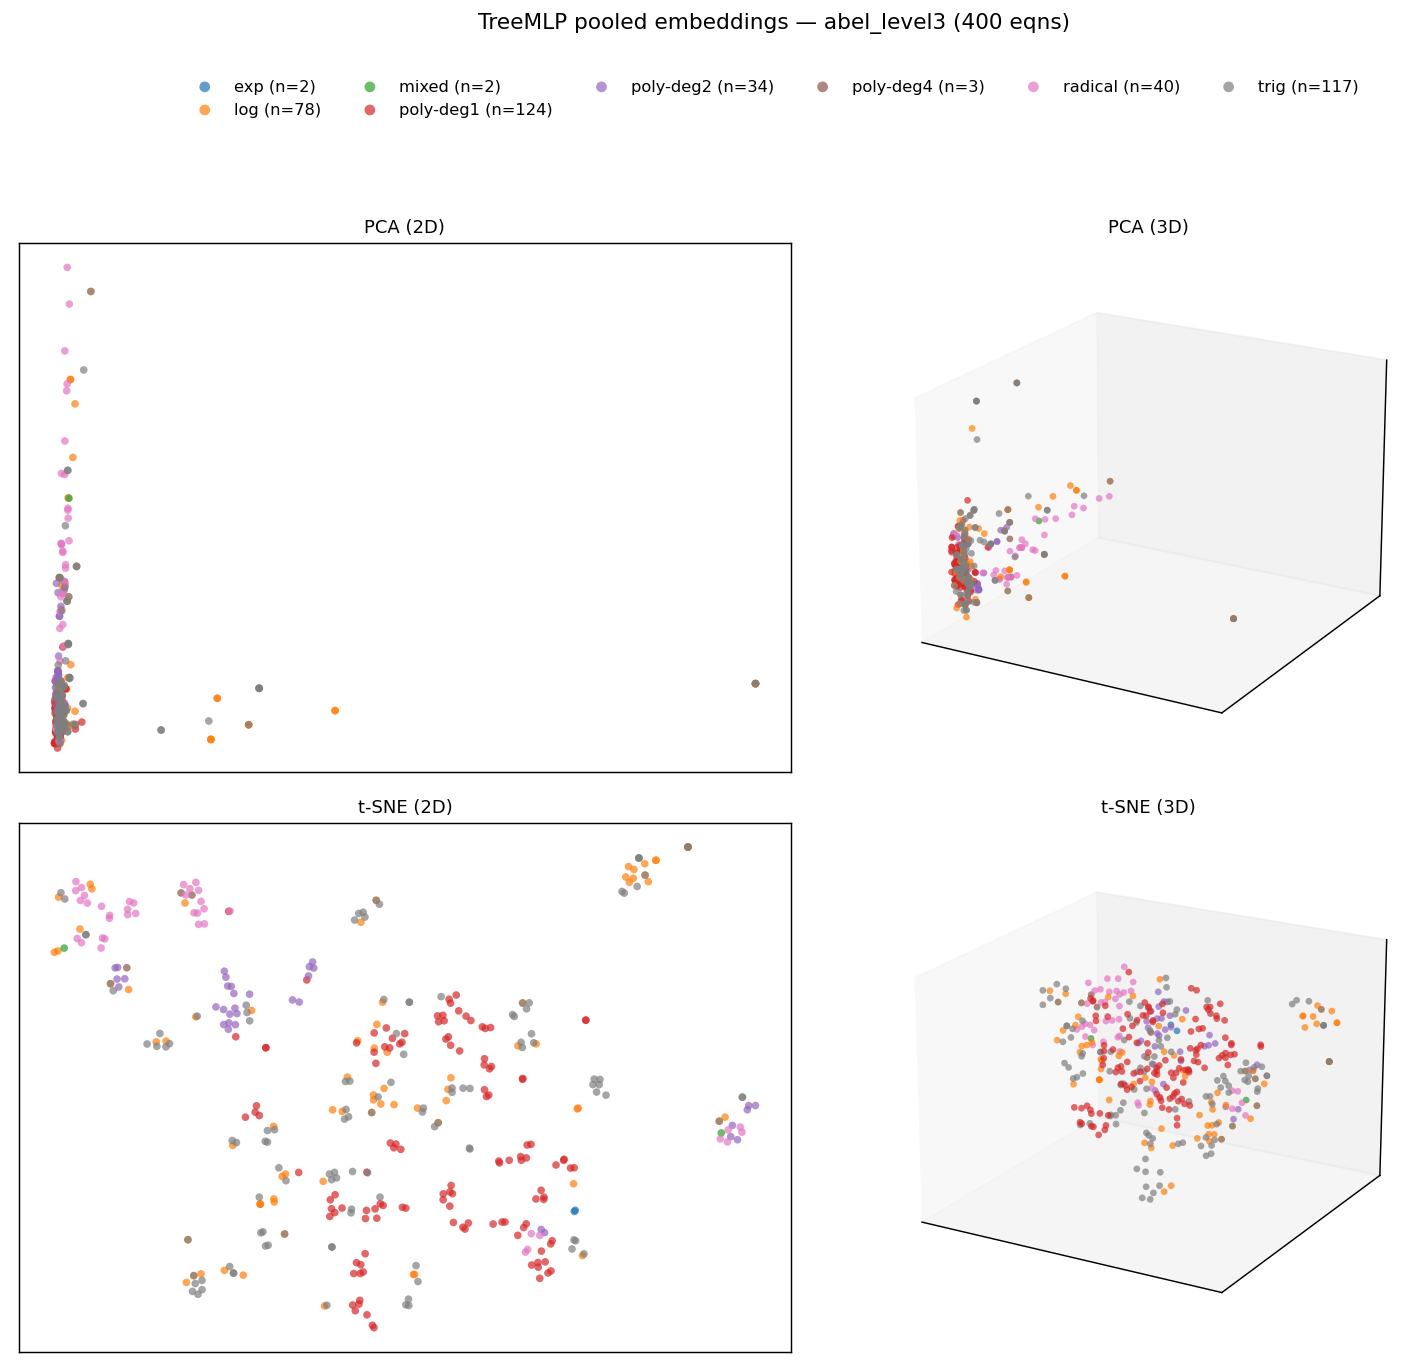
\includegraphics[width=\linewidth]{embed_l3_panel.png}
    \caption{TreeMLP embeddings on the small dataset, projected by PCA (top) and t-SNE (bottom), in 2D (left) and 3D (right). 400 random equations, colored by structural type. The same cluster structure is visible across all four projections.}
    \label{embed_l3_panel}
\end{figure}

\begin{figure}[t]
    \centering
    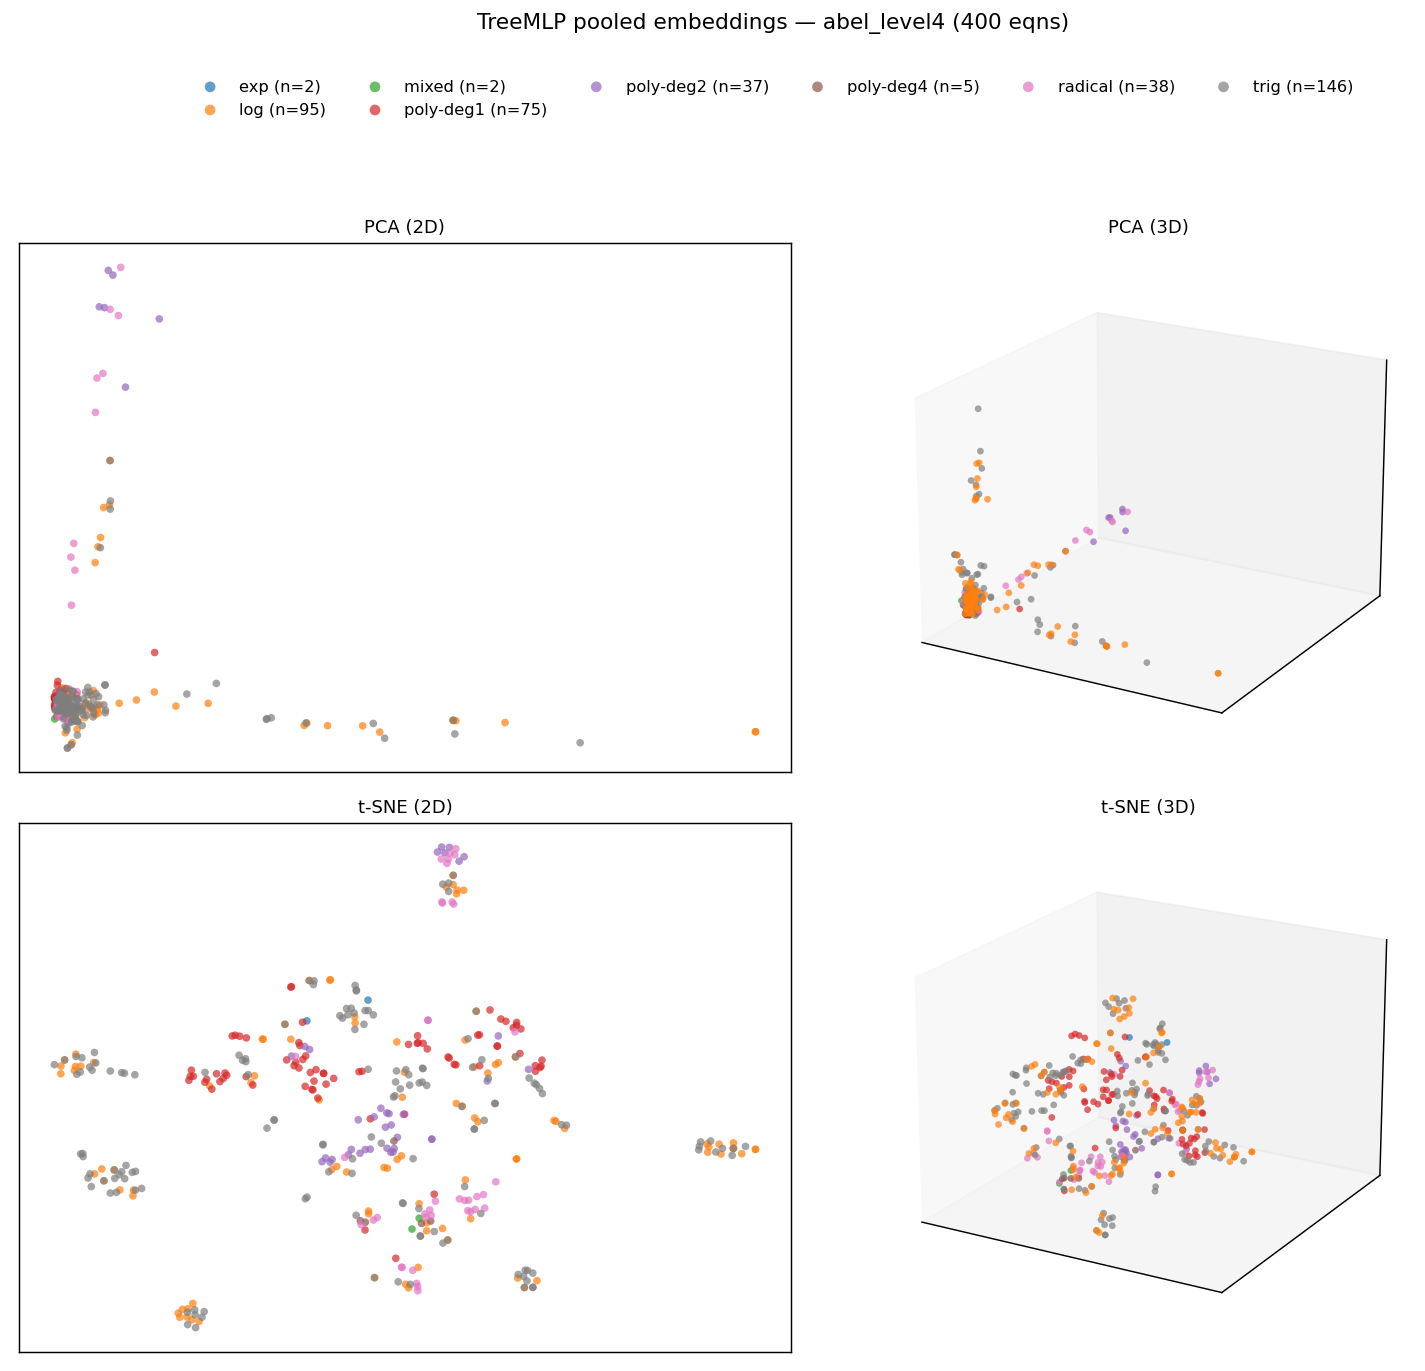
\includegraphics[width=\linewidth]{embed_l4_panel.png}
    \caption{Same as Figure~\ref{embed_l3_panel} but on the large dataset (depth $<5$). More types are present and cluster boundaries are softer, consistent with the lower per-type accuracies reported in the main text.}
    \label{embed_l4_panel}
\end{figure}

\begin{figure}[t]
    \centering
    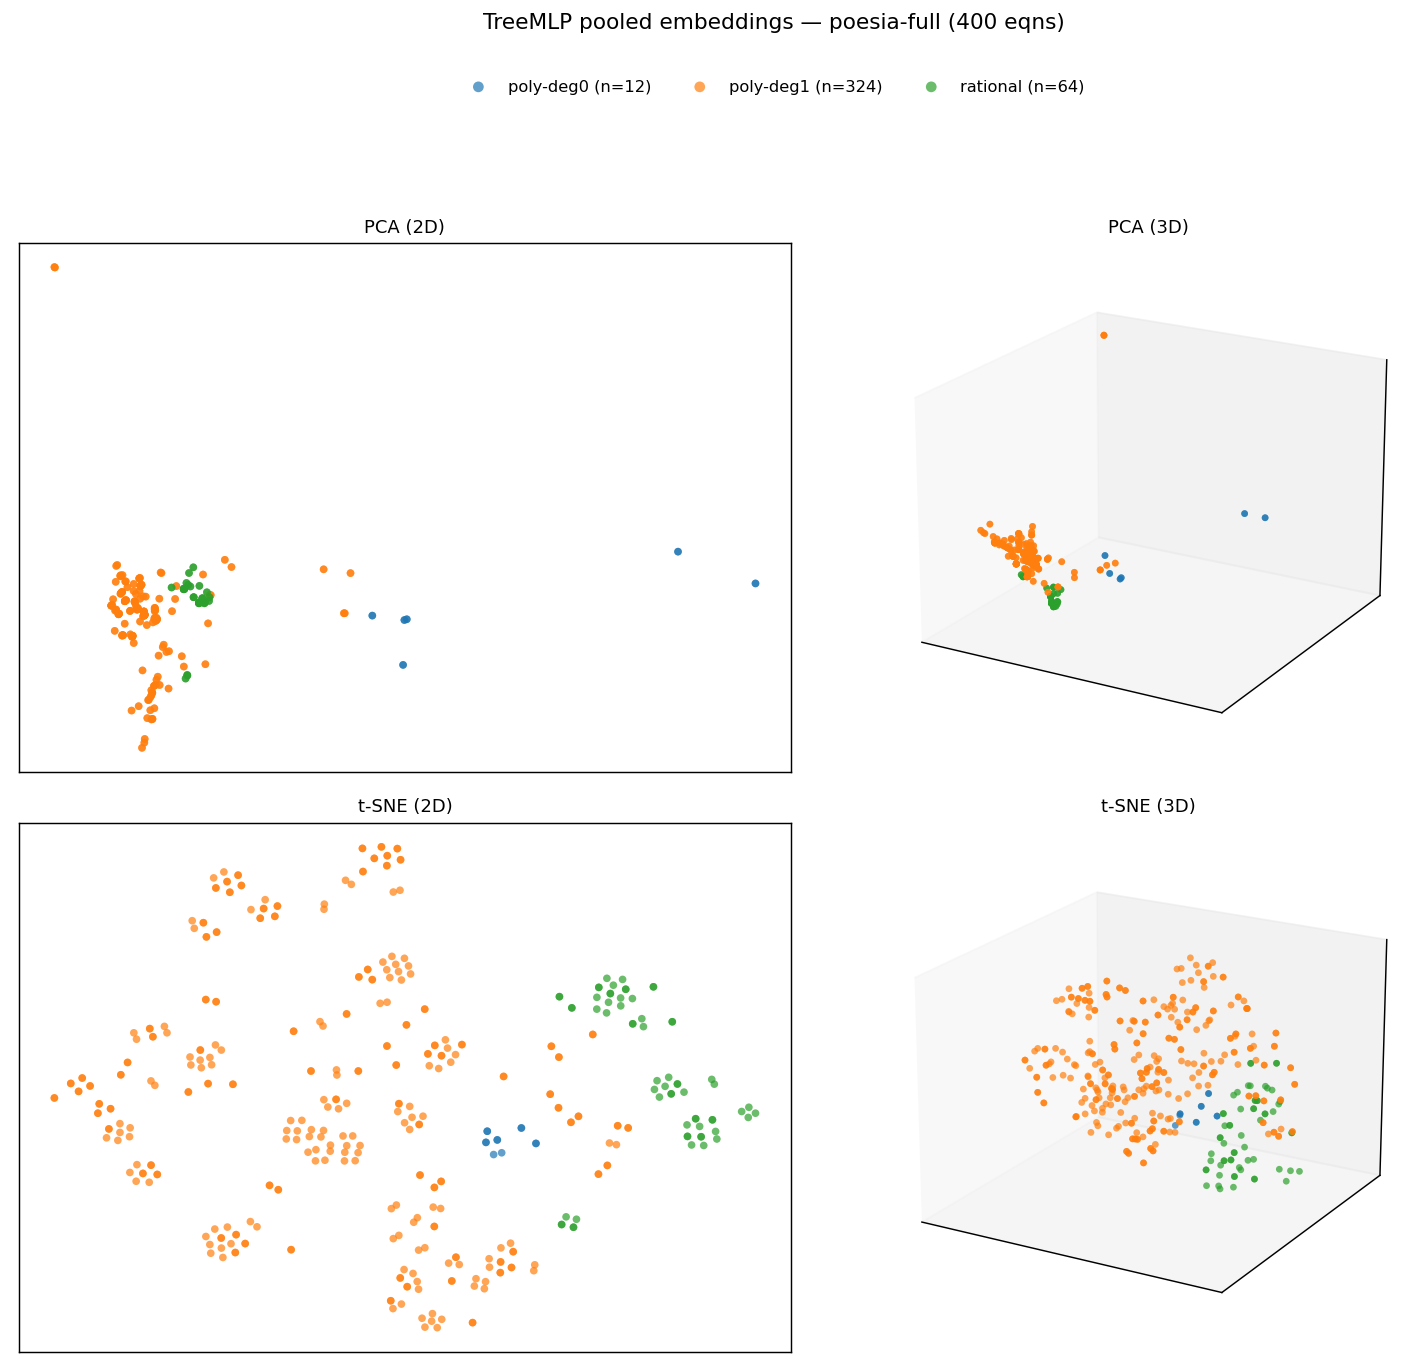
\includegraphics[width=\linewidth]{embed_poesia_panel.png}
    \caption{Same as Figure~\ref{embed_l3_panel} but on CommonCore (poesia). The dataset is dominated by linear and rational equations, giving a simpler embedding geometry.}
    \label{embed_poesia_panel}
\end{figure}


\subsection{Ablations}

We summarize the ablation findings; the corresponding learning curves are in Figures~\ref{ablations} and~\ref{gnn-comparison}.
\begin{itemize}
    \item Replacing dense complexity-delta rewards with sparse outcome-only rewards (and disabling the inverse-frequency curriculum) substantially degrades performance. The main drawback of sparse rewards is \textit{far} longer run times: we had to introduce a 1-second-per-step wall-clock timeout to keep training tractable.
    \item TreeMLP outperforms a vanilla GCN and GraphSAGE on the small dataset (Figure~\ref{gnn-comparison}); the tree-aware aggregation appears necessary, not just helpful.
    \item Curiosity bonuses (ICM, RND, NGU) do not improve TreeMLP learning on \texttt{abel\_level3} (Figure~\ref{curiosity_hurts}). At their full $3\times 10^6$-step horizon, \textsc{icm} and \textsc{ngu} roughly track the no-curiosity baseline on all four metrics (coverage, greedy, beam, success@10); \textsc{rnd} produces a near-flat learning curve, failing to make meaningful progress. This contrasts with earlier work~\cite{dabelow2024symbolic}, where the same family of bonuses \emph{improved} a vanilla MLP policy on a closely related task. A plausible explanation: the TreeMLP's structural inductive bias already supplies the exploration signal that curiosity provides for the MLP, making them redundant or---in the case of \textsc{rnd}---actively conflicting.
\end{itemize}

\begin{figure}[t]
  \centering
  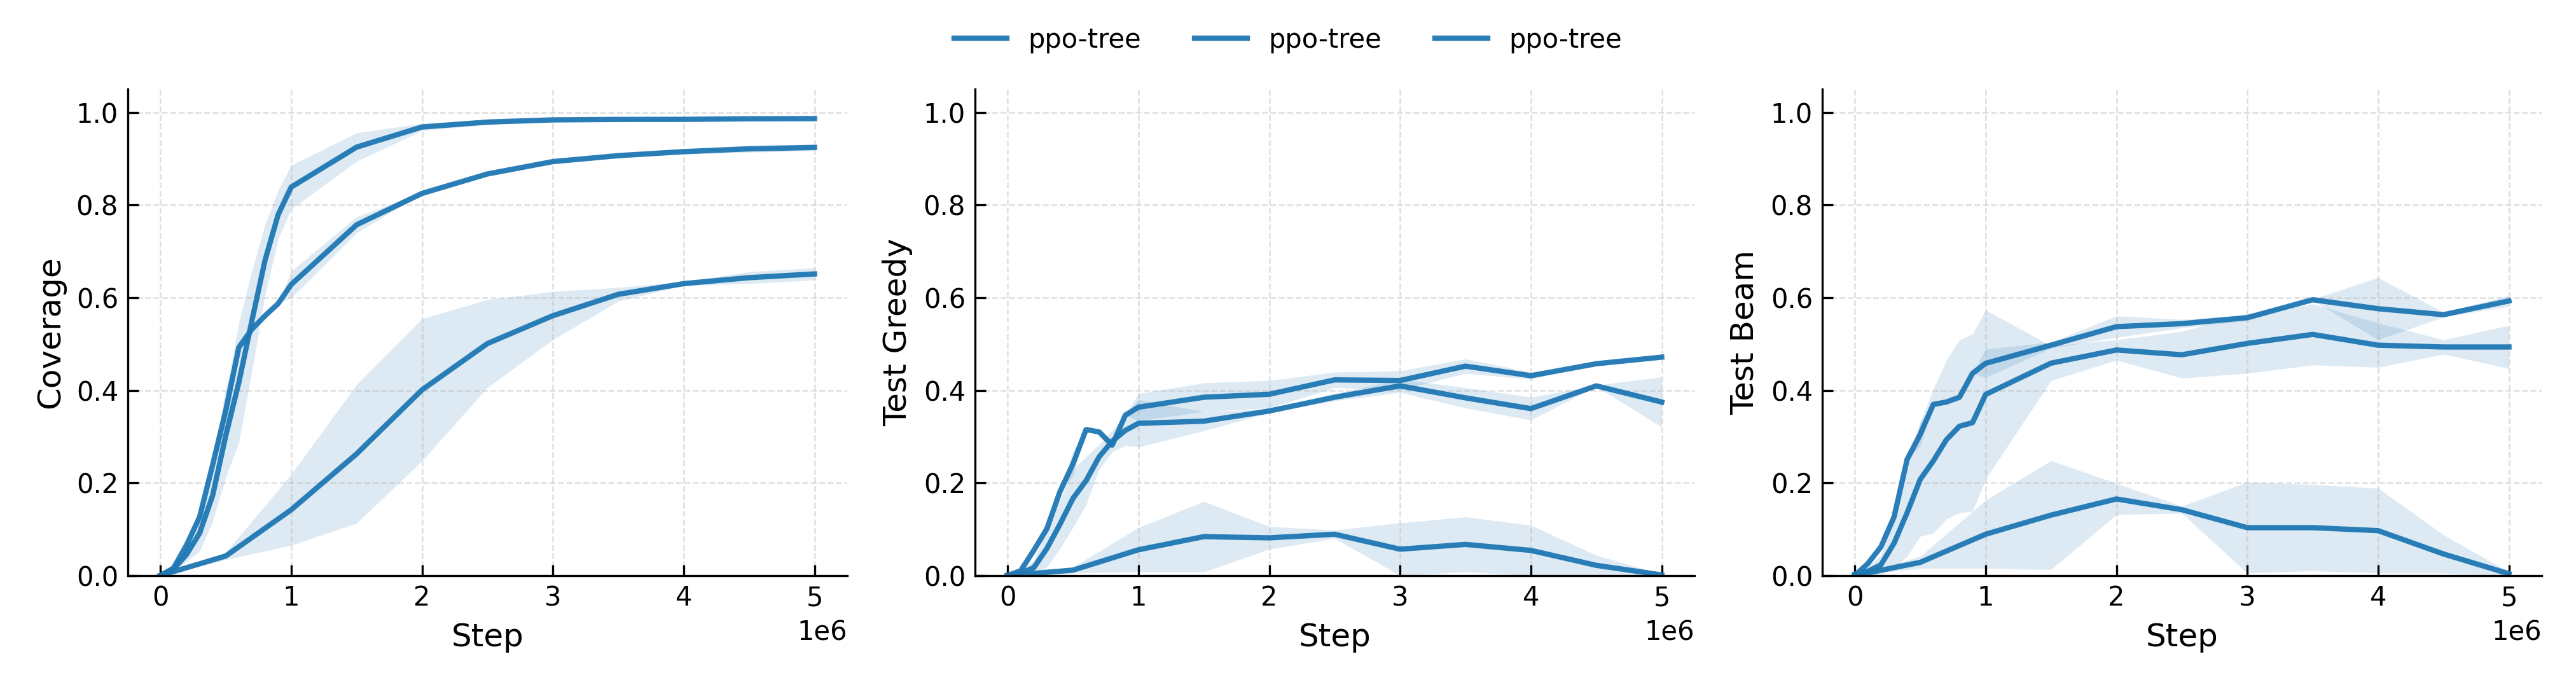
\includegraphics[width=\linewidth]{gnn-comparison.png}
    \caption{TreeMLP outperforms GCN and GraphSAGE on the small datasets. Mean of three random seeds with shading to min/max.}
  \label{gnn-comparison}
\end{figure}


\begin{figure}[t]
  \centering
  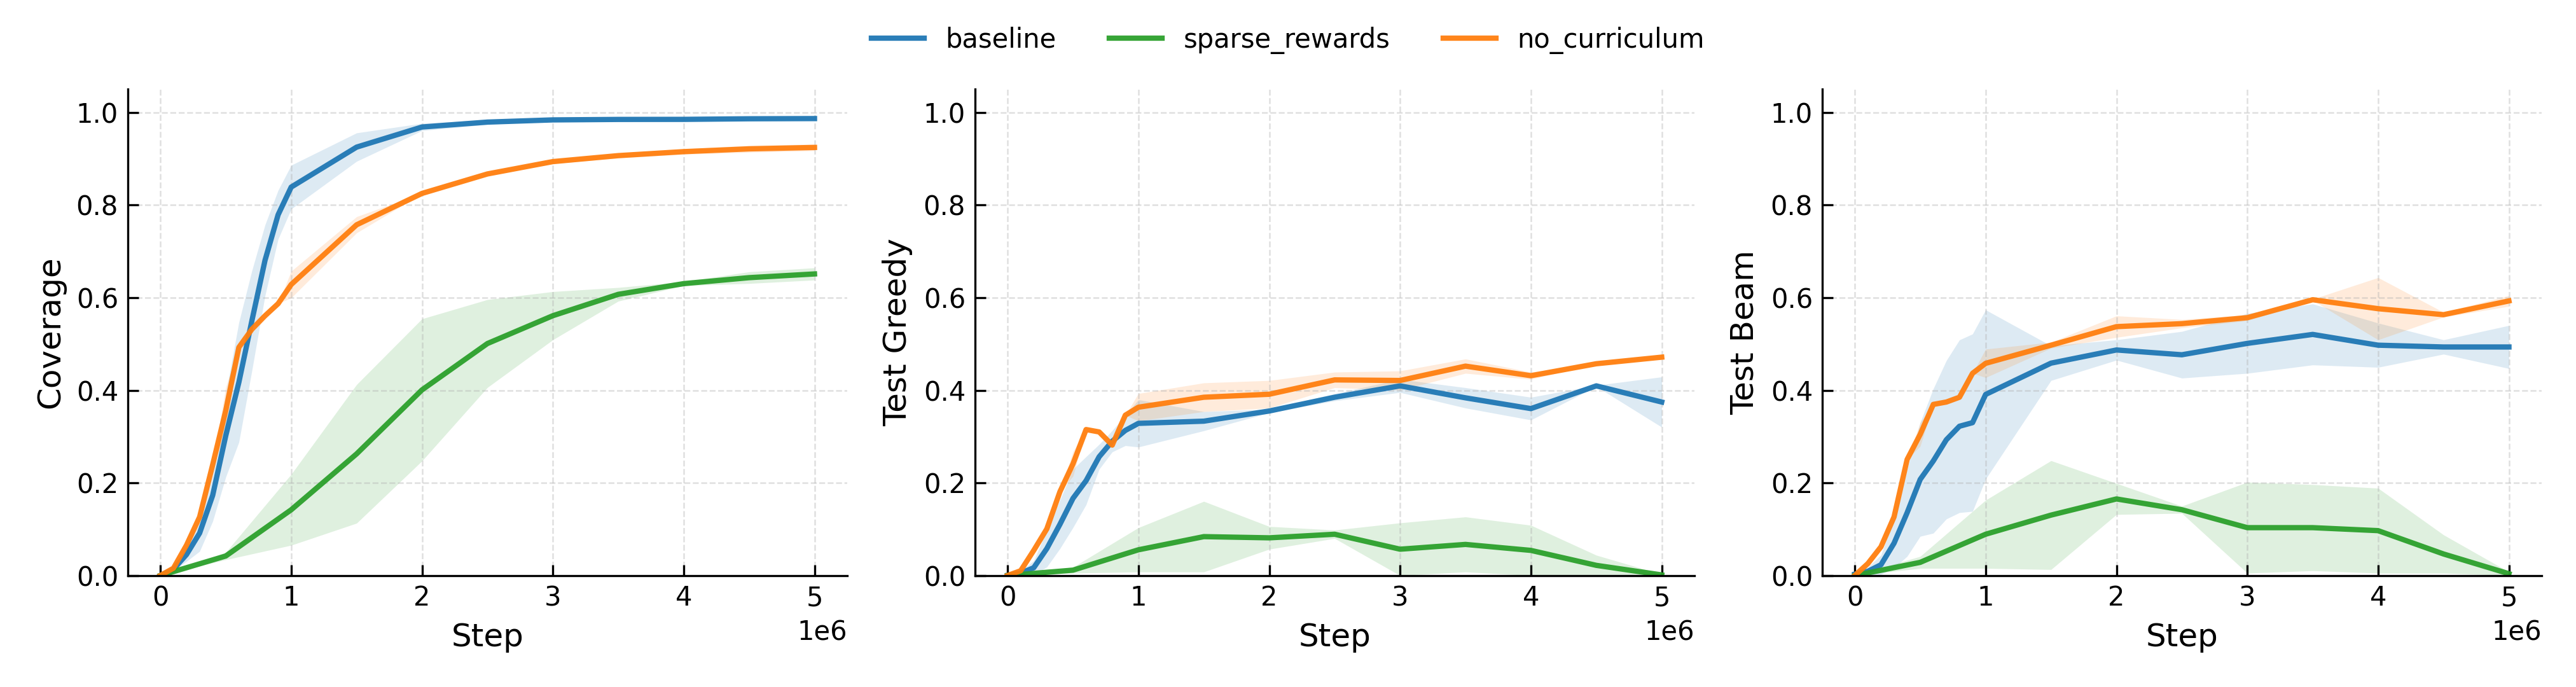
\includegraphics[width=\linewidth]{ablations.png}
    \caption{Ablation study on small datasets.}
  \label{ablations}
\end{figure}

\begin{figure}[t]
  \centering
  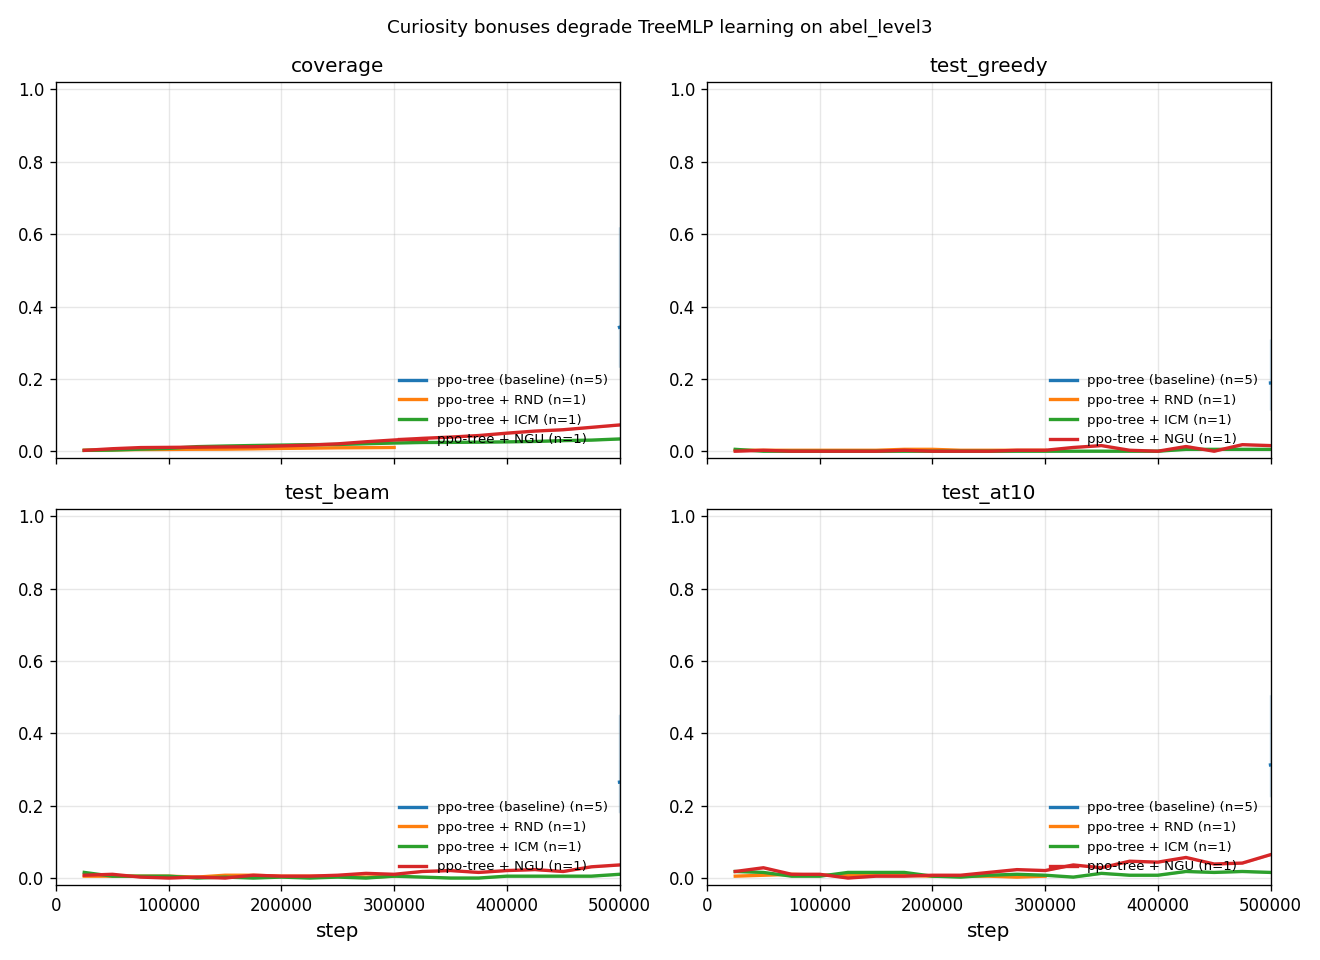
\includegraphics[width=\linewidth]{curiosity-tree-hurts.png}
    \caption{Curiosity bonuses (ICM, NGU, RND) do not improve TreeMLP learning on \texttt{abel\_level3}. At $3{\times}10^6$ steps, \textsc{icm} and \textsc{ngu} roughly track the no-curiosity baseline; \textsc{rnd} produces a near-flat curve. Baseline is mean $\pm$ min/max across $n{=}5$ seeds; curiosity variants are single seed. The previous version of this figure used a $5{\times}10^5$ horizon at which the baseline itself had not yet risen; the difference is now clearly visible.}
  \label{curiosity_hurts}
\end{figure}




\end{document}
